\documentclass{article}
\usepackage[francais]{babel}
\usepackage[utf8]{inputenc}
\usepackage[T1]{fontenc}
\usepackage{graphicx}
%\usepackage{hyperref}

\begin{document}

\title{Projet TPA Manic Shooter \\ Rapport et documentation}
\author{Boutigny Adrien \& Dechipre Matthieu}
%\date\today
\maketitle

\newpage

\tableofcontents

\newpage

\section{Introduction}

Le Manic Shooter est un sous genre de Shoot-em-up, une sorte de jeu de tir dynamique est nerveux à base de bullets et de lasers. Cette sous branche à commencé à vraiment sortir du lot dans les années 90 avec des licences célèbres comme Touhou Project en 1996 ou encore DoDonpachi en 1998, des monuments de ce type de jeu. \newline

Celui-ci se différencie des Shoot-em up classiques par certaines caractéristiques. Tout d'abord, la taille du "vaisseau" du joueur se limite dans la plupart des Manic Shooter à un pixel, pourquoi ? Tout simplement pour pouvoir faire face à la deuxième caractèristique phare du Manic Shooter, la multitude de projectiles qui apparaissent à l'écran comme vous pouvez le voir sur cette image tirée de Touhou Project

\begin{center}
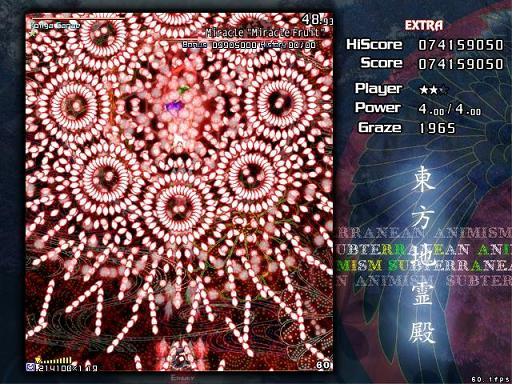
\includegraphics[scale=0.75]{images/touhou_project.jpg}
\end{center}

L'objectif de notre projet est donc le suivant, créer un Manic Shooter. Il faut donc qu'il est les mêmes atouts et défauts que ce dernier. De ce fait, nous avons mis en place un place un moteur de jeu capable de gérer ce nombre immense de projectiles mais aussi d'ennemis. \newline

Dans le cadre de ce jeu, nous avons crée un story-mode, une sorte de mode histoire ou des stages définis à l'avance s'enchainent et où les joueurs pourront tenter d'afficher le highscore. Ce mode se révèle très corsée contrairement au deuxième mode. \newline

Ce deuxième mode en question est un mode où l'on génère de manière procédurale (c'est à dire que l'on imbrique aléatoirement plusieurs vagues d'ennemis prédéfinis) le niveau. Ainsi, en fonction de la difficulté, on obtient un niveau différent à chaque fois. \newline

Suite à plusieurs problèmes, nous avons été obligé de ralentir la progression du jeu et n'avons ajouté des ennemis différents et la gestion du score que très tardivement. La génération de niveau et la majeure partie du moteur de jeu ont été fait pendant le premier semestre et la première moitié du deuxième semestre. \newline

La deuxième moitié du deuxième semestre a été mise à profit pour équilibrer certains ennemis, modifier l'esthétique du jeu, créer de nouveaux ennemis ou encore gérer le highscore et le menu pause. \newline

Nous allons désormais aborder le fonctionnement du jeu et ses mécaniques. \newpage

\section{Fonctionnement}

\subsection{Les menu}

Ce que nous voyons en premier en jouant, ce sont les menus. En effet, dès que le jeu se lance, voici ce à quoi le joueur est confronté:

\begin{center}
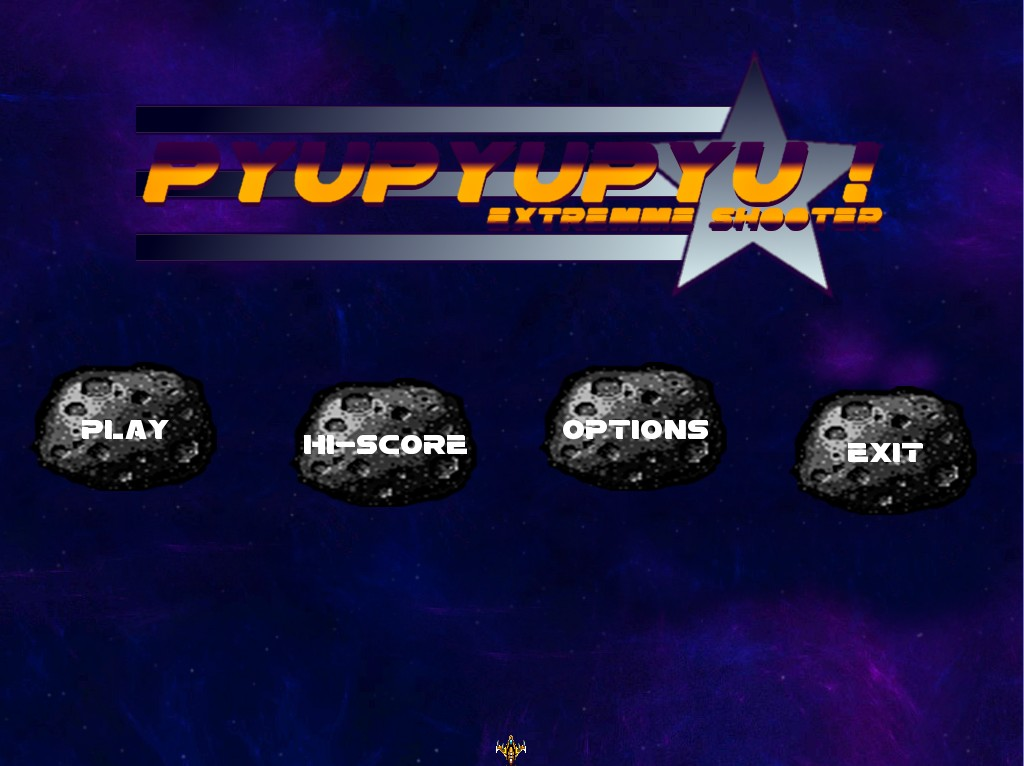
\includegraphics[scale=0.5]{images/menuprinc.jpg}
\end{center}

C'est là que le joueur commence à avoir la main. Il peut bouger le vaisseau via les flèches directionnelles pour se déplacer et tirer sur les astéroïdes afin de choisir ce qu'il veut faire. Chaque astéroïde est en fait un ennemi invincible qui, lorsqu'il se fait toucher, renvoie à une action bien spécifique.

Nous allons maintenant voir ce que fait chacun de ces gros rochers. 

\subsection{Play}

Lorsque le joueur tire sur cette option, un autre menu s'offre à lui avec la possibilité de choisir entre les trois options que vous pouvez voir ici:

\begin{center}
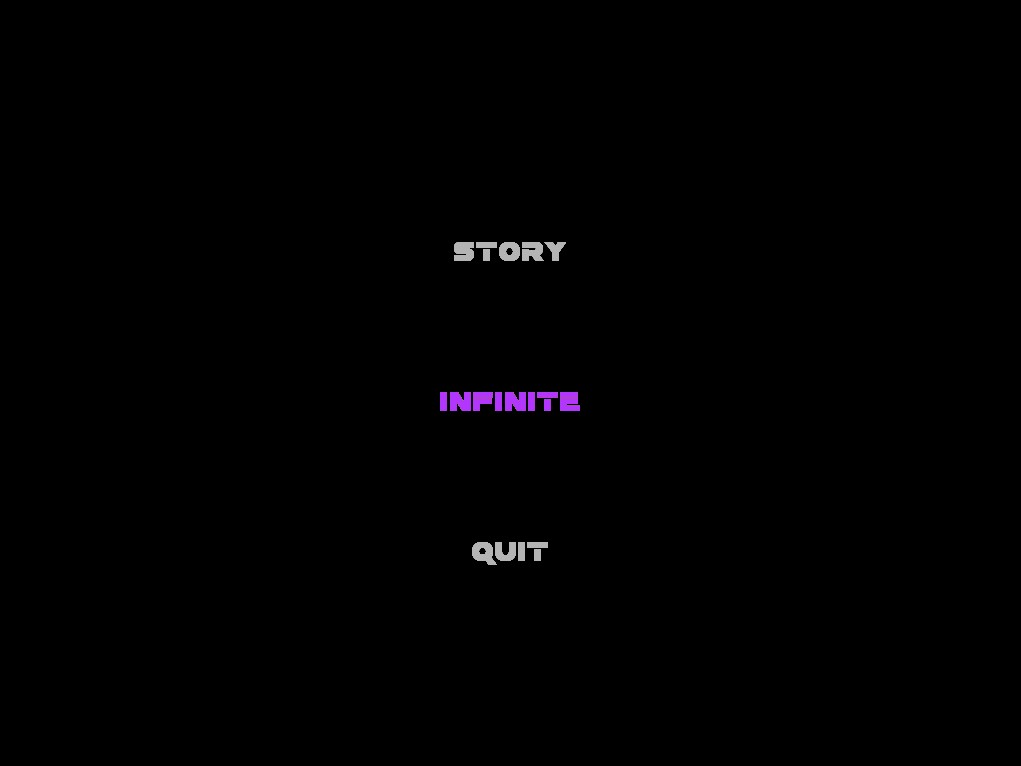
\includegraphics[scale=0.5]{images/sousmenu.jpg}
\end{center}

Les deux premiers sont des modes de jeu et le dernier permet au joueur de revenir au menu principal. Maintenant, voyons ce que propose chaque mode de jeu.

\subsubsection{Mode histoire}

Le mode histoire est un mode très simple qui va simplement amener le joueur à traverser trois niveaux différents avec un boss à la fin de chaque niveau. Les stages ont été conçus à l'avance et permet de découvrir tous les types d'ennemis implémentés dans le jeu. \newline

Les stages se décomposent en blocks qui sont mis bout à bout de manière logique et réfléchi dans ce mode, ce qui n'est pas le cas pour le mode infini, que nous vous allons vous expliquer plus en détail tout comme ces fameux blocks. 

\subsubsection{Le mode infini et le générateur de niveaux}

Pour le mode infini de notre jeu, nous avons crée un générateur de niveaux. Ce générateur de niveau se trouve dans le module level.py de notre dépôt et est constitué de plusieurs classes et fonctions. Ce que ce module fait, c'est prendre le contenu des fichiers exemple.dcbbf qui contiennent donc des blocks d'ennemis et va transformer ces blocks en liste d'ennemis qu'il va ensuite mettre bout à bout de manière aléatoire en fonction d'une difficulté (on choisira seulement les blocks dont la difficulté est inférieure ou égale à la difficulté du niveau généré). \newline

Maintenant que nous avons vu de manière assez simple comment nous générons les niveaux, allons plus dans le détail. Tout d'abord, les fichiers .dcbbf. \newline

Un fichier .dcbbf est un fichier qui contient plusieurs informations selon un format bien précis pour permettre au générateur de niveaux de les traiter correctement. Ces fichiers contiennent: \newline

\begin{itemize}
	\item la difficulté de l'ennemi (1)
	\item le niveau de rareté en fonction de la difficulté (2)
	\item les ennemis (3) \newline
\end{itemize}

Comme vous pouvez le voir ci-dessous sur la capture d'écran d'un fichier block:

\begin{center}
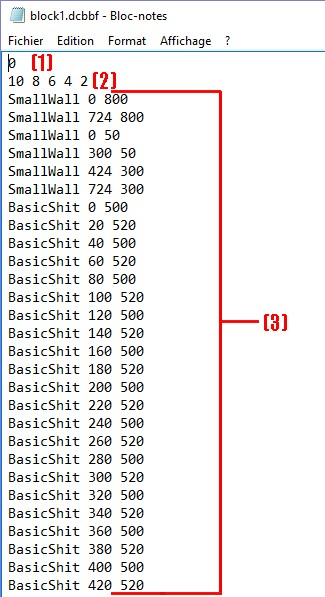
\includegraphics[scale=0.75]{images/explaindcbbf.jpg}
\end{center}

Pour les ennemis normaux, la difficulté va de 0 à 5 et pour les boss de -1 à -5. La difficulté du niveau est aussi l'index qui permettra de définir la rareté du block. En effet, reprenons l'exemple ci-dessus. Si la difficulté choisie pour la création du niveau est de 1, ce block bien précis sera sélectionné car sa difficulté est inférieure à 1. De plus, sa rareté sera fixé à 8 car le générateur va créer une liste de rareté [10, 8, 6, 4, 2] et que l'élément d'indice 1 est 8. Le (3) sera tout simplement la liste des ennemis avec dans l'ordre, le type d'ennemi, la position de sa hitbox en x et la position de sa hitbox en y. \newline

Lorsque l'on voudra créer un niveau, le générateur va charger tous les blocks possibles et ensuite créer deux dictionnaires de fréquence, un pour les blocks standards et un pour ceux des boss. On fait cela car on ne veut qu'un seul boss par niveau à la fin de ce dernier et que de ce fait on ne veut pas qu'il puisse être tiré au hasard parmi les ennemis standards. C'est pour cela que les boss ont des difficulté négatives, on ne s'en sert que pour créer deux dictionnaires différents, sinon, on applique abs(difficulté) - 1 pour pouvoir utiliser correctement leur difficulté. \newline
 
Par la suite, si les blocks ont une difficulté inférieure ou égale à celle du niveau, on les ajoute à leur dictionnaire des fréquences. Pour finir, on va prendre un nombre de blocks aléatoires en fonction de leurs fréquences d'apparition et on va créer une liste d'ennemis à partir des ennemis que le block contient. \newline

Pour finir, nous parlerons de la gestion des positions des ennemis dans les blocks. Vous avez pu le constater dans l'exemple, tous les ennemis ont leur position en y inférieur à 1000, et les autres fichiers d'ennemis sont pareils. C'est parce que chaque block contient des ennemis sur 1000 pixels, pas plus. Il faut donc prendre ça en compte lorsque nous créons la liste d'ennemis. Pour le premier block, on ne change rien, pour le deuxième block, on ajoute 1000px à tous les ennemis en y, 2000 pour le troisième etc ...

Le schéma ci-dessous résume le processus:

\begin{center}
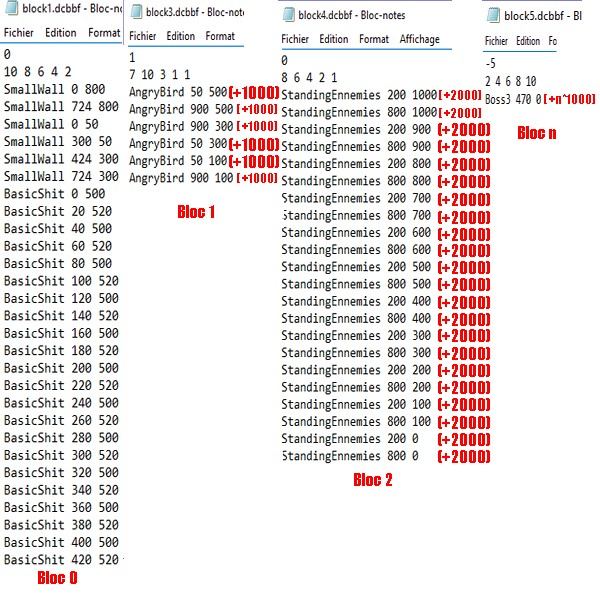
\includegraphics[scale=0.75]{images/explaindcbbf2.jpg}
\end{center}

Comme le générateur fonctionne actuellement, le mode Infini de notre jeu fonctionne par vague de 20 blocks avec un boss à la fin de chaque vague. La difficulté commence à 0 et augmente d'un cran tous les 20 blocks jusqu'à un maximum de 4.

\subsection{Hi-Score}

La partie consacré à Play étant terminé, à quoi sert l'astéroïde suivant. Lorsque le joueur tire dessus, celui-ci accède à un écran des scores semblable à celui-ci:

\begin{center}
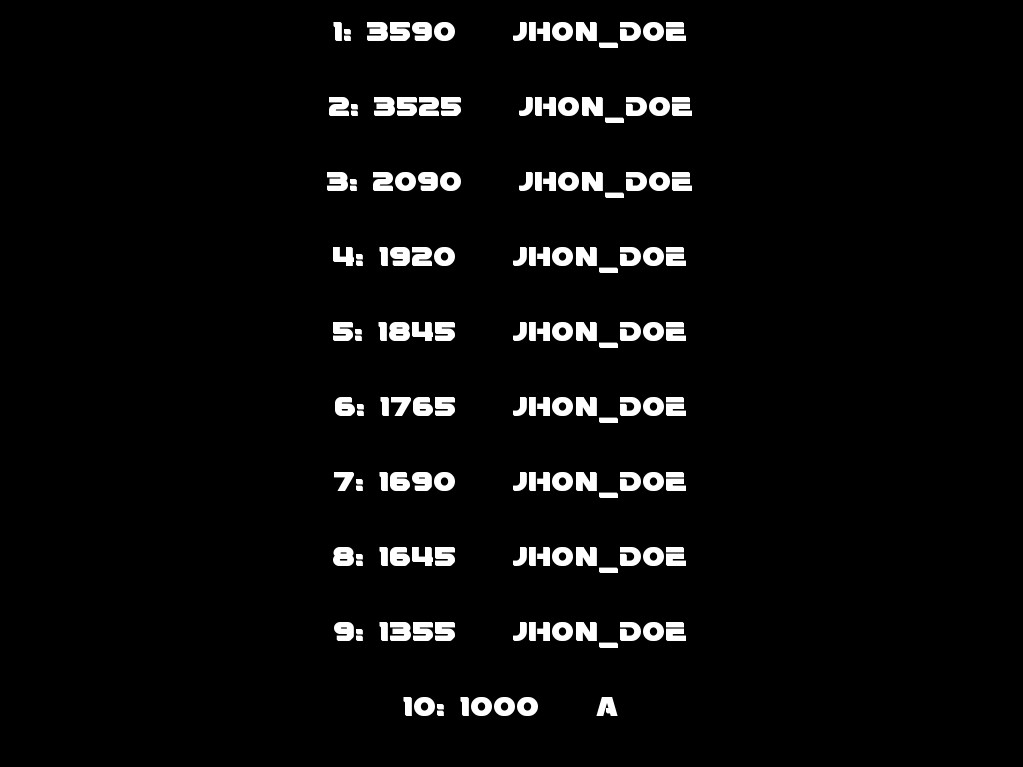
\includegraphics[scale=0.5]{images/hiscore.jpg}
\end{center}

Le joueur peut alors observer les meilleurs scores atteints par les autres joueurs avant lui. Il y a donc le score suivi du nom de celui qui l'a effectué. Malheureusement pour l'instant il n'y a pas la possibilité d'entrer un nom donc il n'y en aura qu'un seul par défaut, à savoir Jhon\_Doe. \newline

Les scores et noms présents dans ce classement se trouvent dans un fichier à part, story\_score.txt. Quand l'utilisateur tire sur le Hi-Score, la fonction load\_score présente dans le module misc.py va être utilisé pour charger les données du fichiers à partir de la classe Score présente dans le même fichier. \newline

Quand le joueur finira le mode histoire, son score sera gardé en mémoire et donc enregistré dans le fichier de score. Le score le plus bas sera détruit car nous ne conservons que 10 scores en mémoire maximum.

\subsection{Exit}

Comme son nom l'indique, quand le joueur tire dessus, le jeu s'arrête et l'utilisateur quitte donc l'application.

\subsection{Le jeu}

\subsubsection{Les collisions}

Nous utilisons uniquement des collisions à base de rectangles.
Le coût peu élevé de l'algorithme nous arrange car nous avons parfois des
centaines de collisions à tester à chaque frame. \newline


Cet algorithme peut s'exprimer facilement avec l'illustration tirée du
site développez.com suivante. Ici, le bleu est avant la ligne jaune minimum du
rouge, bleu et rouge ne sont pas en collision et le jaune est avant le maximum
du rouge, ils sont en collision:

\begin{center}
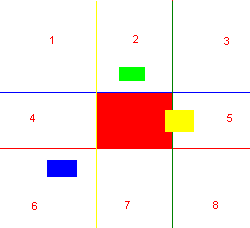
\includegraphics[scale= 0.8]{images/collision-boites.png}
\end{center}

Il est à noter que la hitbox des vaisseaux n'est pas forcément exactement le vaisseau lui-même. En effet, pour l'exemple ci-dessous, la hitbox n'est pas du tout la même que le sprite du vaisseau (la hitbox est rayée en rouge):

\begin{center}
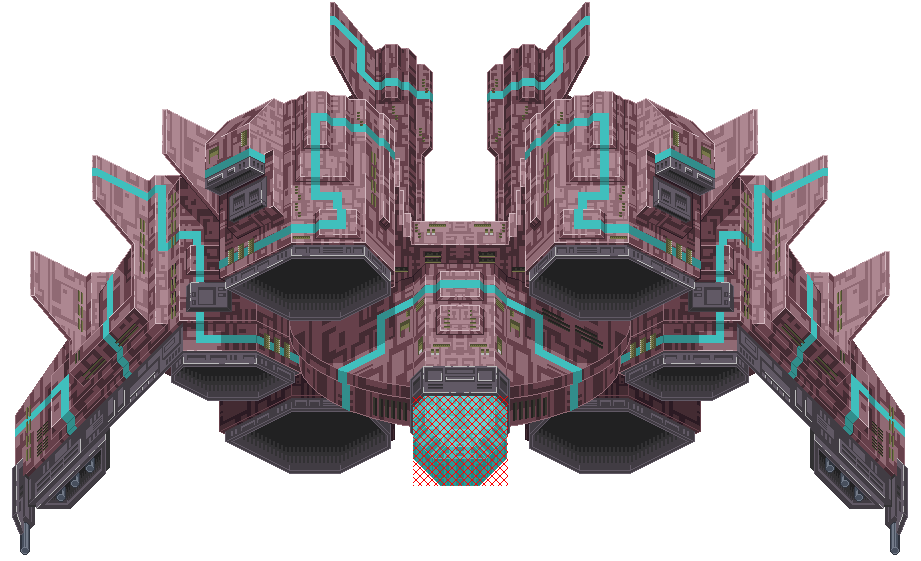
\includegraphics[scale= 0.4]{images/carrierhit.png}
\end{center}

\subsubsection{Les powers-up}

\subsubsection{Recovery-time}

A la différence des vaisseaux ennemis, le joueur doit, s'il a plusieurs vies, avoir le temps de se remettre lorsqu'il est touché. En effet, si le joueur se fait touché par un tir et qu'il se refait toucher un quart de seconde plus tard, ce sera tout simplement frustrant pour lui. \newline

Nous avons donc mis en place une mécanique de jeu de shoot, le recovery time. C'est un temps plus ou moins court qui survient après que le joueur ce soit fait toucher. Pendant cet intervalle, le joueur devient insensible aux dégâts et peut donc se repositionner sans craindre de mourir instantanément. \newline

Ce temps de recouvrement se traduit à l'écran par le clignotement du vaisseau joueur. \newpage

\section{Organisation }

\newpage

\section{Réalisation}

\subsection{Environnement}

Nous avons utilisé plusieurs langage de programmation, bibliothèques et outils lors de la création de ce jeu, à savoir: \newline

- Python 3, notre langage de programmation principale, celui avec lequel nous avons crée tout le jeu \newline

- Pysdl2, une librairie dépendante de Python 3 et descendante de Sdl2 qui nous a permis de gérer tout le multimédia de notre application, à savoir les graphismes, les bruitages et ambiance sonore \newline

- Divers logiciels de traitement d'images afin de créer les sprites, les retoucher etc ... Comme Gimp ou encore Photofiltre \newline

- Des outils de création sonore 8-bits comme bfxr dont le lien se trouve dans la partie source de ce compte-rendu   

\subsection{Répartition du travail}

Au tout début du projet, nous étions quatre à travailler dessus. Très vite, le groupe se réduisit à trois personnes. Nous avons réparti le travail parmi nous. L'un s'occupait principalement de la boucle principale, l'un des vaisseaux et l'autre de tout ce qui était lié au vaisseaux. \newline

Le premier semestre se déroula donc ainsi à trois, malgré la répartition des tâches, chacun regardait très souvent ce que faisait les autres et y apportait des modifications ou créait de nouvelles choses. \newline

Et le deuxième semestre transforma notre groupe en binôme. Et nous avons travaillé à ce moment à rendre le jeu plus jouable et plus agréable, avec un menu pauses, deux modes de jeu et en travaillant à rendre plus nombreux et différents les ennemis possibles.

\newpage

\section{Conclusion: apports et critiques}

\newpage

\section{Suppléments}

\subsection{Sources}

\noindent https://www.libsdl.org/ \newline
https://www.python.org/download/releases/3.4.0/ \newline
http://www.bfxr.net/ \newline 
http://www.photofiltre-studio.com/news.htm \newline
https://www.gimp.org/


\subsection{Documentation}

\noindent http://www.developpez.com/ \newline
https://openclassrooms.com/ \newline
https://pysdl2.readthedocs.org/en/latest/

\end{document}
